\documentclass[11pt]{article}

\usepackage[margin=1in]{geometry}
\usepackage[T1]{fontenc}
\usepackage[utf8]{inputenc}
\usepackage{lmodern}
\usepackage{microtype}
\usepackage{amsmath,amssymb,amsthm,mathtools}
\usepackage{bm}
\usepackage{booktabs}
\usepackage{enumitem}
\usepackage{tikz}
\usepackage{xcolor}
\usepackage[numbers,sort&compress]{natbib}
\usepackage[colorlinks=true,linkcolor=blue!60!black,citecolor=blue!60!black,urlcolor=blue!60!black]{hyperref}

\usetikzlibrary{arrows.meta,positioning,calc}

\newtheorem{definition}{Definition}[section]
\newtheorem{proposition}[definition]{Proposition}
\newtheorem{corollary}[definition]{Corollary}
\theoremstyle{remark}
\newtheorem{remark}[definition]{Remark}

\newcommand{\R}{\mathbb{R}}
\newcommand{\C}{\mathbb{C}}
\newcommand{\HH}{\mathbb{H}}
\newcommand{\CP}{\mathbb{CP}}
\newcommand{\SU}{\mathrm{SU}}
\newcommand{\U}{\mathrm{U}}
\newcommand{\SO}{\mathrm{SO}}
\newcommand{\Sp}{\mathrm{Sp}}
\newcommand{\ii}{\mathbf{i}}
\newcommand{\jj}{\mathbf{j}}
\newcommand{\kk}{\mathbf{k}}
\newcommand{\transpose}{\mathsf{T}}
\newcommand{\adjoint}{^\dagger}
\newcommand{\inv}{^{-1}}
\newcommand{\tr}{\operatorname{tr}}
\newcommand{\Id}{I}
\newcommand{\norm}[1]{\left\lVert #1 \right\rVert}
\newcommand{\abs}[1]{\left\lvert #1 \right\rvert}
\newcommand{\set}[1]{\left\{ #1 \right\}}
\newcommand{\ket}[1]{\lvert #1 \rangle}
\newcommand{\bra}[1]{\langle #1 \rvert}
\newcommand{\inner}[2]{\langle #1, #2 \rangle}
\newcommand{\bloch}[1]{\bm{#1}}
\newcommand{\qvec}{\mathbf{u}}

\title{\textbf{Foundations of Quaternionic Quantum Computing:}\\
Qubits, Spinors, and $\SU(2)$ Geometry}

\author{RQM Technologies Research Team\thanks{Organizational author record used for this draft. Individual author records are pending confirmation. Correspondence: \texttt{research@rqm-technologies.com}.}\\
RQM Technologies}

\date{Version 0.1.0 \\ Draft dated 2026-04-09}

\begin{document}
\maketitle

\begin{abstract}
This paper assembles a conservative mathematical foundation for the use of quaternions in single-qubit quantum computing. The goal is not to replace standard quantum mechanics, but to organize familiar structures in a way that makes their geometry more explicit. We distinguish carefully between normalized state vectors in $\C^2 \cong \R^4$, the unit sphere $S^3$ inside that space, pure states modulo global phase, the projective space $\CP^1 \cong S^2$, the single-qubit gate group $\U(2)$, and $\SU(2)$ representatives obtained after removing global phase. Within that framework, we exhibit an explicit isomorphism between the unit quaternions and $\SU(2)$, explain why unit quaternions are therefore a natural model for single-qubit gates modulo global phase, and show how quaternion multiplication exposes the axis--angle and composition structure of rotations. Standard facts are separated from the organizational choices adopted in the RQM Technologies series. The paper is restricted to single-qubit structure and makes no claim about new physics, multi-qubit quaternionic state evolution, or computational advantage.
\end{abstract}

\noindent\textbf{Keywords:} qubit geometry; spinors; $\SU(2)$; unit quaternions; Bloch sphere; single-qubit gates

\section{Introduction}

Single-qubit quantum mechanics is usually presented in matrix language: states are vectors in $\C^2$, observables are Hermitian matrices, and gates are unitary matrices. That formulation is complete and standard. The issue addressed here is not a defect in quantum mechanics itself, but a question of representation. In particular, some geometric features of single-qubit dynamics are more transparent when one passes from raw $2 \times 2$ complex matrices to the equivalent language of unit quaternions.

The connection is classical. A normalized two-component spinor is a point on the unit sphere in $\C^2 \cong \R^4$, hence on $S^3$. The group $\SU(2)$ is also diffeomorphic to $S^3$. Unit quaternions form another model of the same manifold and, more strongly, a Lie-group model of $\SU(2)$ \citep{hall2015,kuipers1999,penrose1984}. For single-qubit gates this is not an exotic reformulation: it is standard mathematics attached to the well-known double cover $\SU(2)\to\SO(3)$.

The main value of the quaternionic presentation is geometric bookkeeping. In matrix form, one can certainly write
\[
U = \cos(\theta/2)\Id - i \sin(\theta/2)\,(\hat{\bloch{n}}\cdot\bm{\sigma}),
\]
but the composition law remains hidden inside matrix multiplication. In quaternion form, the same gate is written as
\[
q = \cos(\theta/2) + \sin(\theta/2)\,(n_x \ii + n_y \jj + n_z \kk),
\]
and the product law immediately exhibits dot and cross products. This makes the rotation structure of single-qubit gates unusually explicit.

The scope of this paper is deliberately narrow. It treats only the mathematics needed to explain why quaternions belong naturally in \emph{single-qubit} quantum computing. It does not argue for quaternionic Hilbert spaces as a new physical theory, and it does not claim any hardware or complexity-theoretic advantage. The purpose is foundational exposition: to present standard structures with clear distinctions, and to identify exactly which interpretive or organizational choices belong to RQM Technologies rather than to established mathematics.

\section{Mathematical preliminaries}

\subsection{Qubits as normalized vectors in \texorpdfstring{$\C^2$}{C2}}

A pure single-qubit state is represented by a nonzero vector
\[
\ket{\psi}=\begin{pmatrix}\alpha \\ \beta\end{pmatrix}\in \C^2,
\]
with the physical state unchanged under multiplication by a nonzero complex scalar. After normalization one may assume
\[
\abs{\alpha}^2+\abs{\beta}^2=1.
\]
The normalized representatives are often called normalized spinors.

Writing
\[
\alpha=a+ib,\qquad \beta=c+id,\qquad a,b,c,d\in\R,
\]
identifies $\C^2$ with $\R^4$.

\begin{proposition}[Normalized spinors form $S^3$]
The set
\[
\set{(\alpha,\beta)\in\C^2:\abs{\alpha}^2+\abs{\beta}^2=1}
\]
is the unit sphere $S^3\subset \R^4$ under the identification $\C^2\cong\R^4$.
\end{proposition}

\begin{proof}
Under $\alpha=a+ib$ and $\beta=c+id$, the normalization condition becomes
\[
a^2+b^2+c^2+d^2=1,
\]
which is exactly the defining equation of the unit $3$-sphere in $\R^4$.
\end{proof}

\begin{remark}
This $S^3$ is a space of \emph{normalized representatives}. It is not yet the physical pure-state space, because global phase has not been quotiented out.
\end{remark}

\subsection{Pure states, global phase, and the Bloch sphere}

Two normalized vectors $\ket{\psi}$ and $e^{i\chi}\ket{\psi}$ represent the same pure state. The pure-state space is therefore the projective quotient
\[
\CP^1 = \big(\C^2\setminus\set{0}\big)/\C^\times,
\]
or, after normalization, the quotient of $S^3$ by the circle action
\[
(\alpha,\beta)\mapsto(e^{i\chi}\alpha,e^{i\chi}\beta).
\]

\begin{proposition}[Pure single-qubit states are $\CP^1\cong S^2$]
The pure-state space of a single qubit is $\CP^1$, and $\CP^1$ is diffeomorphic to $S^2$. Under this identification the Bloch vector of
\[
\ket{\psi}=\begin{pmatrix}\alpha \\ \beta\end{pmatrix}
\]
is
\[
\bloch{r}(\psi)=
\bigl(2\operatorname{Re}(\alpha^\ast\beta),\,
2\operatorname{Im}(\alpha^\ast\beta),\,
\abs{\alpha}^2-\abs{\beta}^2\bigr)\in S^2.
\]
\end{proposition}

\begin{proof}
The quotient description of $\CP^1$ is standard. For normalized $\ket{\psi}$, a direct calculation shows
\[
\norm{\bloch{r}(\psi)}^2
=4\abs{\alpha^\ast\beta}^2+\bigl(\abs{\alpha}^2-\abs{\beta}^2\bigr)^2
=\bigl(\abs{\alpha}^2+\abs{\beta}^2\bigr)^2=1.
\]
The map $\ket{\psi}\mapsto\bloch{r}(\psi)$ is invariant under $\ket{\psi}\mapsto e^{i\chi}\ket{\psi}$, so it descends to the projective quotient and yields the usual identification of $\CP^1$ with the Bloch sphere $S^2$ \citep{bloch1946,nielsen2010}.
\end{proof}

\begin{remark}
The Bloch sphere is therefore a quotient of the state sphere $S^3$. It is \emph{not} the same object as $S^3$, and conflating the two obscures the role of global phase.
\end{remark}

\subsection{Single-qubit gates in \texorpdfstring{$\U(2)$}{U(2)} and representatives in \texorpdfstring{$\SU(2)$}{SU(2)}}

Single-qubit gates are unitary operators on $\C^2$, hence elements of $\U(2)$. Because a global phase on the state vector is physically irrelevant, two gates that differ by an overall phase act identically on pure states.

\begin{proposition}[Removing global phase from a single-qubit gate]
For every $U\in\U(2)$ there exist $\chi\in\R$ and $V\in\SU(2)$ such that
\[
U=e^{i\chi}V.
\]
The representative $V$ is unique up to multiplication by $-1$.
\end{proposition}

\begin{proof}
Since $\det U\in \U(1)$, choose $\chi$ such that $e^{2i\chi}=\det U$, and define $V=e^{-i\chi}U$. Then
\[
\det V=e^{-2i\chi}\det U=1,
\]
so $V\in\SU(2)$. If also $U=e^{i\chi'}V'$ with $V'\in\SU(2)$, then
\[
V' = e^{i(\chi-\chi')}V.
\]
Taking determinants gives $e^{2i(\chi-\chi')}=1$, hence $e^{i(\chi-\chi')}=\pm 1$ and $V'=\pm V$.
\end{proof}

Thus physically distinct single-qubit gate actions are represented projectively by
\[
\U(2)/\U(1)\cong \SU(2)/\set{\pm\Id}\cong \SO(3),
\]
while it is often convenient to work with a chosen representative in $\SU(2)$ before passing to the projective quotient.

\subsection{Unit quaternions}

\begin{definition}
The quaternion algebra $\HH$ is the real associative algebra with basis $\set{1,\ii,\jj,\kk}$ and multiplication rules
\[
\ii^2=\jj^2=\kk^2=\ii\jj\kk=-1.
\]
Every quaternion has the form
\[
q=a+b\ii+c\jj+d\kk,\qquad a,b,c,d\in\R.
\]
Its conjugate is $\overline{q}=a-b\ii-c\jj-d\kk$, and its norm is
\[
\abs{q}=\sqrt{q\overline{q}}=\sqrt{a^2+b^2+c^2+d^2}.
\]
\end{definition}

The unit quaternions are
\[
\Sp(1)=\set{q\in\HH:\abs{q}=1}.
\]
As a manifold, $\Sp(1)$ is again $S^3$.

\begin{remark}
At this point two appearances of $S^3$ coexist:
\begin{enumerate}[label=(\roman*)]
\item normalized spinors in $\C^2$, and
\item unit quaternions, equivalently $\Sp(1)$.
\end{enumerate}
They are diffeomorphic manifolds, but they play different semantic roles: the first is a space of normalized vectors, while the second is a group of transformations. The distinction matters throughout the paper.
\end{remark}

\section{The \texorpdfstring{$\SU(2)$}{SU(2)}--unit-quaternion correspondence}

\subsection{An explicit map}

There are several equivalent conventions for identifying $\HH$ with a real subalgebra of $2\times2$ complex matrices. In this paper we choose the convention
\begin{equation}
\Phi(a+b\ii+c\jj+d\kk)
=
\begin{pmatrix}
a-di & -c-bi\\
c-bi & a+di
\end{pmatrix}.
\label{eq:phi}
\end{equation}
Equivalently,
\[
\Phi(q)=a\Id-i\bigl(b\sigma_x+c\sigma_y+d\sigma_z\bigr),
\]
where $\sigma_x,\sigma_y,\sigma_z$ are the Pauli matrices. This convention is convenient because the quaternion basis units align directly with the $x$-, $y$-, and $z$-rotation axes:
\[
\Phi(\ii)=-i\sigma_x,\qquad \Phi(\jj)=-i\sigma_y,\qquad \Phi(\kk)=-i\sigma_z.
\]

\begin{proposition}[Unit quaternions are isomorphic to $\SU(2)$]
The restriction of $\Phi$ to $\Sp(1)$ is a Lie-group isomorphism
\[
\Phi:\Sp(1)\xrightarrow{\sim}\SU(2).
\]
\end{proposition}

\begin{proof}
The assignment is determined by
\[
\ii\mapsto -i\sigma_x,\qquad
\jj\mapsto -i\sigma_y,\qquad
\kk\mapsto -i\sigma_z.
\]
These matrices satisfy the same multiplication rules as $\ii,\jj,\kk$:
\[
(-i\sigma_x)^2=(-i\sigma_y)^2=(-i\sigma_z)^2=-\Id,
\]
and
\[
(-i\sigma_x)(-i\sigma_y)=-i\sigma_z,
\]
with cyclic permutations. Hence $\Phi$ is an algebra homomorphism and therefore a group homomorphism on invertible elements.

For $q=a+b\ii+c\jj+d\kk$, direct calculation gives
\[
\det \Phi(q)=a^2+b^2+c^2+d^2=\abs{q}^2.
\]
If $\abs{q}=1$, then $\det\Phi(q)=1$ and $\Phi(q)\adjoint\Phi(q)=\Id$, so $\Phi(q)\in\SU(2)$. Conversely, any matrix in $\SU(2)$ has the form
\[
\begin{pmatrix}
\alpha & \beta\\
-\beta^\ast & \alpha^\ast
\end{pmatrix},
\qquad \abs{\alpha}^2+\abs{\beta}^2=1,
\]
and writing $\alpha=a-di$, $\beta=-c-bi$ recovers a unique unit quaternion $a+b\ii+c\jj+d\kk$. Smoothness of $\Phi$ and $\Phi^{-1}$ is immediate from the coordinate formula.
\end{proof}

\begin{corollary}[Composition corresponds to quaternion multiplication]
If $q_1,q_2\in\Sp(1)$ represent single-qubit gates through \eqref{eq:phi}, then sequential application of the gates corresponds to quaternion multiplication:
\[
\Phi(q_2q_1)=\Phi(q_2)\Phi(q_1).
\]
\end{corollary}

\begin{proof}
This is the homomorphism property of $\Phi$.
\end{proof}

\subsection{Why this is the right language for gates modulo global phase}

By the previous section, every physical single-qubit gate class may be represented by an element of $\SU(2)$, unique up to sign, and $\SU(2)$ is modeled exactly by the unit quaternions. It follows that unit quaternions are a natural representation of single-qubit gates \emph{after} global phase has been factored out at the level of $\U(2)$.

\begin{remark}
This statement must be kept precise. Gates live fundamentally in $\U(2)$. The quaternion model does not replace $\U(2)$; rather, it provides a convenient model of the $\SU(2)$ representative chosen after removing overall phase. The remaining identification $q\sim -q$ corresponds to the fact that $\pm V\in\SU(2)$ induce the same rotation on the Bloch sphere.
\end{remark}

\section{Quaternionic geometry and rotation structure}

\subsection{Axis--angle form}

Every $V\in\SU(2)$ can be written as
\begin{equation}
V=\cos(\theta/2)\Id-i\sin(\theta/2)(\hat{\bloch{n}}\cdot\bm{\sigma}),
\label{eq:axis-angle-su2}
\end{equation}
where $\hat{\bloch{n}}=(n_x,n_y,n_z)\in S^2$ and $\theta\in\R$. Under \eqref{eq:phi}, the corresponding quaternion is
\begin{equation}
q=\cos(\theta/2)+\sin(\theta/2)(n_x\ii+n_y\jj+n_z\kk).
\label{eq:axis-angle-quaternion}
\end{equation}
This is the standard axis--angle form of a unit quaternion \citep{kuipers1999,hall2015}.

The familiar Pauli rotations are immediate:
\[
R_x(\theta)\leftrightarrow \cos(\theta/2)+\sin(\theta/2)\ii,
\]
\[
R_y(\theta)\leftrightarrow \cos(\theta/2)+\sin(\theta/2)\jj,
\]
\[
R_z(\theta)\leftrightarrow \cos(\theta/2)+\sin(\theta/2)\kk.
\]
In particular, $\pi$-rotations correspond, up to global phase, to the basis units $\ii,\jj,\kk$.

\subsection{Composition as scalar--vector algebra}

Write a quaternion as $q=a+\qvec$, where $a\in\R$ and $\qvec=b\ii+c\jj+d\kk$ is its pure part, identified with a vector in $\R^3$. Then quaternion multiplication becomes
\begin{equation}
(a_1+\qvec_1)(a_2+\qvec_2)
=
\bigl(a_1a_2-\qvec_1\cdot\qvec_2\bigr)
\;+\;
\bigl(a_1\qvec_2+a_2\qvec_1+\qvec_1\times\qvec_2\bigr).
\label{eq:scalar-vector}
\end{equation}
Equation \eqref{eq:scalar-vector} makes three features transparent:
\begin{enumerate}[label=(\alph*)]
\item the scalar part records the dot product of the pure parts;
\item the pure part contains the cross product responsible for noncommutativity; and
\item sequential gate composition is visibly a rotation-composition law, not merely an abstract matrix product.
\end{enumerate}

This is one sense in which quaternionic notation clarifies geometry that matrix notation can hide. The matrix formulation already contains the same information, but it is encoded less directly.

\subsection{The double cover \texorpdfstring{$\SU(2)\to\SO(3)$}{SU(2) to SO(3)}}

The action of a unit quaternion on a pure quaternion $v=x\ii+y\jj+z\kk$ by conjugation,
\[
v\longmapsto qvq^{-1},
\]
preserves the pure-quaternion subspace and its Euclidean norm. Identifying pure quaternions with $\R^3$ therefore gives a homomorphism
\[
\rho:\Sp(1)\to\SO(3).
\]

\begin{proposition}[Unit quaternions double-cover $\SO(3)$]
The map $\rho$ is surjective and has kernel $\set{\pm1}$. Consequently,
\[
\Sp(1)/\set{\pm1}\cong \SO(3).
\]
Via $\Phi$, the same statement is the familiar double cover $\SU(2)\to\SO(3)$.
\end{proposition}

\begin{proof}
The conjugation action preserves multiplication and the norm on pure quaternions, hence lands in $\SO(3)$. Standard rotation theory shows that every element of $\SO(3)$ admits an axis--angle lift of the form \eqref{eq:axis-angle-quaternion}, establishing surjectivity. If $qvq^{-1}=v$ for every pure quaternion $v$, then $q$ commutes with all pure quaternions, which forces $q\in\R$. Since $q$ is unitary, $q=\pm1$.
\end{proof}

\begin{remark}
The sign ambiguity here should not be confused with global phase for state vectors, although the two are related. A $2\pi$ rotation in $\SO(3)$ lifts to a path in $\SU(2)$ from $\Id$ to $-\Id$, so spinors return to the same physical pure state only projectively. This is standard spin-$1/2$ geometry \citep{penrose1984}.
\end{remark}

\section{What is standard mathematics, and what is RQM framing?}

\subsection{Standard facts used in this paper}

The following statements are standard and not specific to RQM Technologies:
\begin{enumerate}[label=(\arabic*)]
\item normalized vectors in $\C^2$ form $S^3$;
\item pure single-qubit states are projective classes, giving $\CP^1\cong S^2$;
\item single-qubit gates live in $\U(2)$;
\item after removal of overall phase, gates admit representatives in $\SU(2)$;
\item the unit quaternions form a Lie group isomorphic to $\SU(2)$;
\item $\SU(2)$ is a double cover of $\SO(3)$; and
\item axis--angle rotations can be written equivalently in Pauli-matrix form or quaternion form.
\end{enumerate}
These are standard results from quantum mechanics, Lie theory, and quaternionic rotation theory \citep{nielsen2010,hall2015,kuipers1999,penrose1984}.

\subsection{RQM Technologies framing choices}

The project-specific content of this paper is modest and organizational:
\begin{enumerate}[label=(\alph*)]
\item \textbf{Primary expository emphasis.} The paper chooses the quaternion model as the preferred language for describing \emph{single-qubit gate geometry}.
\item \textbf{Convention choice.} The explicit map $\Phi$ in \eqref{eq:phi} is selected so that $\ii,\jj,\kk$ align with the $x,y,z$ Pauli axes. This is one standard convention among several equivalent ones.
\item \textbf{Series organization.} The paper serves as a terminology and notation baseline for later papers in the series.
\end{enumerate}

These are framing choices, not new physical claims. They do not alter the content of standard single-qubit quantum mechanics.

\section{Scope, limitations, and non-claims}

This paper is intentionally limited. In particular, it makes the following non-claims explicit:
\begin{enumerate}[label=(\arabic*)]
\item It does \emph{not} claim that standard complex-matrix methods are inadequate or invalid.
\item It does \emph{not} claim a new physical theory or a replacement of ordinary quantum mechanics.
\item It does \emph{not} claim a hardware implementation advantage.
\item It does \emph{not} claim a complexity-theoretic or algorithmic advantage.
\item It does \emph{not} develop a multi-qubit quaternionic state formalism.
\item It does \emph{not} treat quaternionic Hilbert-space quantum mechanics in the sense studied by \citet{adler1995}; that subject is distinct from the present gate-level representation question.
\end{enumerate}

The paper should therefore be read as a clarifying foundation for single-qubit language only.

\section{Conclusion}

For a single qubit, the relevant geometry links together several standard structures:
\begin{itemize}
\item normalized spinors in $\C^2$, forming $S^3$;
\item pure states modulo global phase, forming $\CP^1\cong S^2$;
\item single-qubit gates in $\U(2)$, with $\SU(2)$ representatives after removing global phase; and
\item unit quaternions as an explicit Lie-group model of $\SU(2)$.
\end{itemize}
The quaternion model is therefore natural not because it changes the theory, but because it presents the existing rotation structure of single-qubit gates in a compact geometric form. In that sense, quaternions belong naturally in single-qubit quantum computing as a representation language for $\SU(2)$ and its relation to the Bloch sphere.

\appendix

\section{Notation used repeatedly}

\begin{center}
\begin{tabular}{@{}lll@{}}
\toprule
Symbol & Meaning & Role \\
\midrule
$\ket{\psi}$ & normalized state vector in $\C^2$ & state representative \\
$S^3$ & unit sphere in $\C^2\cong\R^4$ & normalized spinors \\
$\CP^1$ & projective pure-state space & pure states modulo phase \\
$S^2$ & Bloch sphere & pure states / Bloch vectors \\
$U$ & element of $\U(2)$ & single-qubit gate \\
$V$ & representative in $\SU(2)$ & gate modulo global phase \\
$q$ & unit quaternion & model of $V\in\SU(2)$ \\
$\Phi$ & quaternion--matrix identification & convention chosen here \\
\bottomrule
\end{tabular}
\end{center}

\section{Schematic figures}

\begin{figure}[h]
\centering
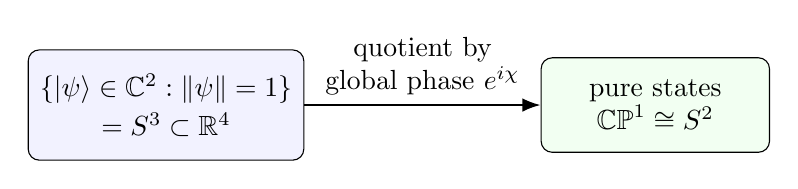
\begin{tikzpicture}[node distance=1.8cm, >=Latex]
  \node[draw, rounded corners, minimum width=3.5cm, minimum height=1.4cm, align=center, fill=blue!5] (spinor) {$\{\ket{\psi}\in\C^2:\norm{\psi}=1\}$\\[2pt]$=S^3\subset\R^4$};
  \node[draw, rounded corners, minimum width=2.9cm, minimum height=1.2cm, right=3cm of spinor, align=center, fill=green!5] (projective) {pure states\\$\CP^1\cong S^2$};
  \draw[->, thick] (spinor) -- node[above, align=center] {quotient by\\global phase $e^{i\chi}$} (projective);
\end{tikzpicture}
\caption{Normalized spinors form $S^3$, while pure states arise only after quotienting by global phase. The resulting space is $\CP^1\cong S^2$, the Bloch sphere.}
\end{figure}

\begin{figure}[h]
\centering
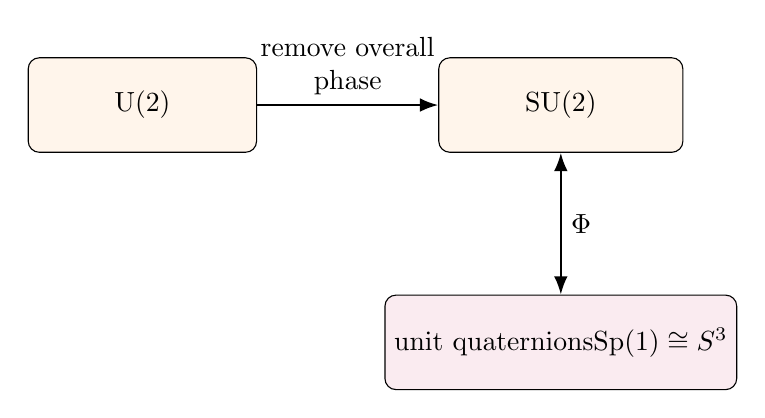
\begin{tikzpicture}[node distance=2.0cm, >=Latex]
  \node[draw, rounded corners, minimum width=2.9cm, minimum height=1.2cm, fill=orange!8] (u2) {$\U(2)$};
  \node[draw, rounded corners, minimum width=3.1cm, minimum height=1.2cm, right=2.3cm of u2, fill=orange!8] (su2) {$\SU(2)$};
  \node[draw, rounded corners, minimum width=3.5cm, minimum height=1.2cm, below=1.8cm of su2, fill=purple!8] (quat) {unit quaternions\\$\Sp(1)\cong S^3$};
  \draw[->, thick] (u2) -- node[above, align=center] {remove overall\\phase} (su2);
  \draw[<->, thick] (su2) -- node[right] {$\Phi$} (quat);
\end{tikzpicture}
\caption{Single-qubit gates live in $\U(2)$. After removing global phase, one may choose representatives in $\SU(2)$, which are modeled exactly by unit quaternions.}
\end{figure}

\begin{figure}[h]
\centering
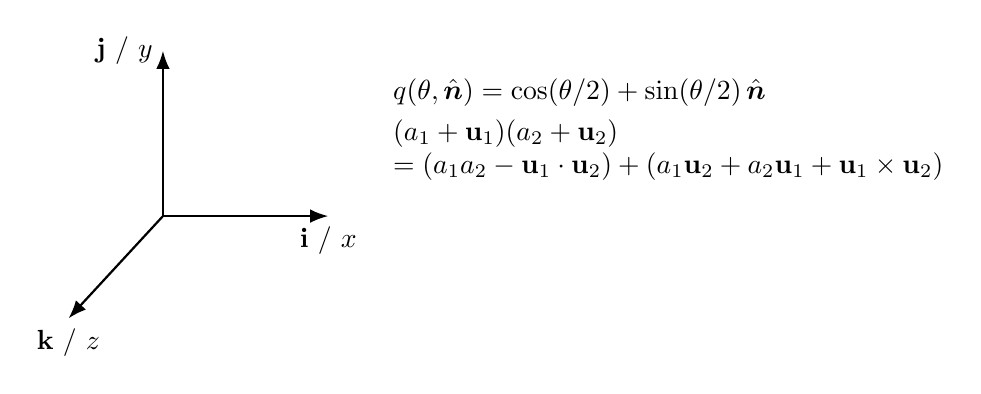
\begin{tikzpicture}[>=Latex]
  \draw[->, thick] (0,0) -- (2.1,0) node[below] {$\ii$ / $x$};
  \draw[->, thick] (0,0) -- (0,2.1) node[left] {$\jj$ / $y$};
  \draw[->, thick] (0,0) -- (-1.2,-1.3) node[below] {$\kk$ / $z$};
  \node[align=left, anchor=west] at (2.8,1.1) {$q(\theta,\hat{\bloch{n}})=\cos(\theta/2)+\sin(\theta/2)\,\hat{\bloch{n}}$\\[3pt]
  $(a_1+\qvec_1)(a_2+\qvec_2)$\\
  $=(a_1a_2-\qvec_1\cdot\qvec_2)+(a_1\qvec_2+a_2\qvec_1+\qvec_1\times\qvec_2)$};
\end{tikzpicture}
\caption{Quaternion coordinates make axis--angle data and rotation composition explicit. The cross-product term records the noncommutativity of sequential rotations.}
\end{figure}

\clearpage
\bibliographystyle{plainnat}
\bibliography{references}

\end{document}
